\chapter{Models on the Hourly Consumption}
In this section, a more detailed look at the hourly consumption will be provided. One of the goals is to get a better understanding of the tap-water consumption during the summer period, such that it can be used when looking at the winter period. This can be done by looking at the distributions of the consumption during the day in the two periods. Another goal of this section is to model the hourly consumption as a time series. An ARIMAX model will be applied to give a better understanding of the data. The ARIMAX model can also be used to give short term predictions of the consumption. These predictions will be compared to the ones provided by the multiple regression model.


\begin{figure}
    \centering
    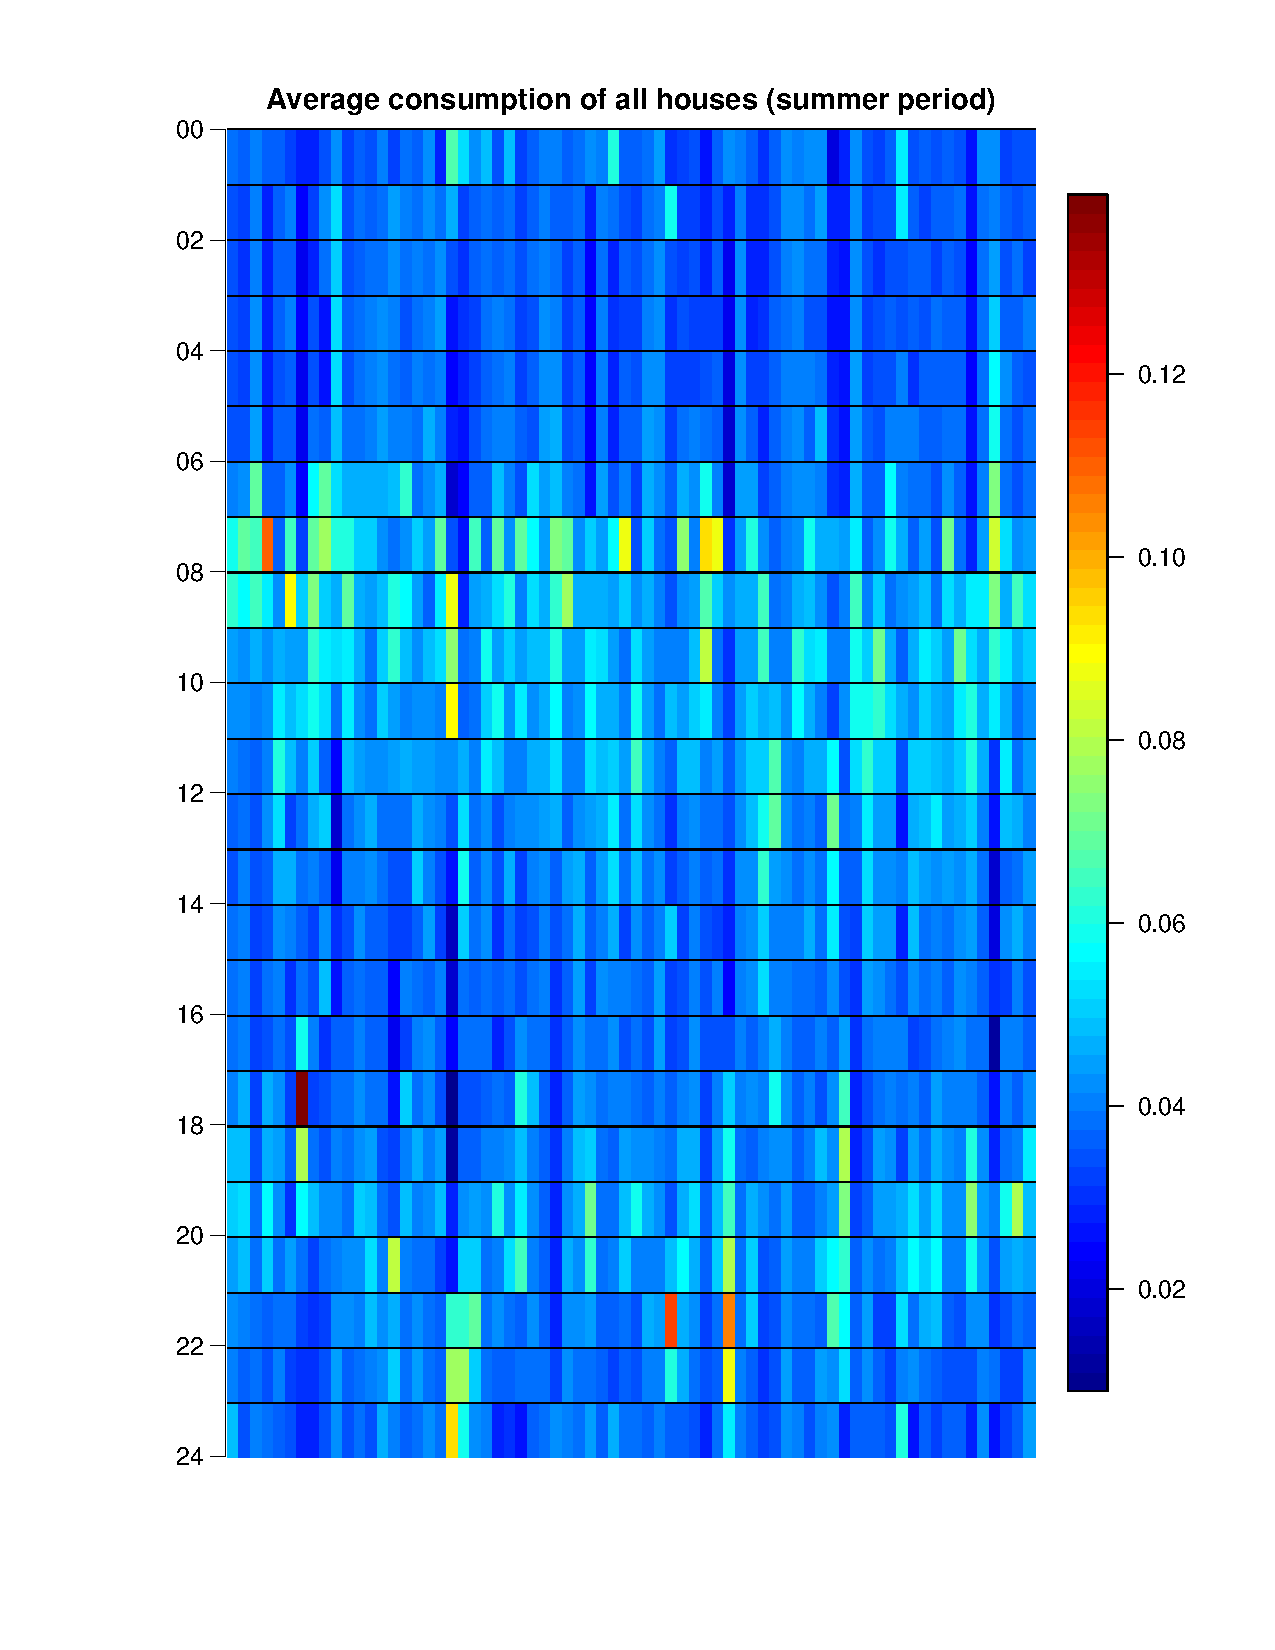
\includegraphics[width=\textwidth]{../../../figures/Heatmap_summer.pdf}
    \caption{The normalized average consumption of every house during the day in the summer period. This is characterized by the days where the average outside temperature is above 15 degrees. The horizontal lines indicate the hours and each vertical strip is a house. The scale indicates the fraction of the total consumption during the day}
    \label{fig: Hourcons_summer}
\end{figure}


\begin{figure}
    \centering
    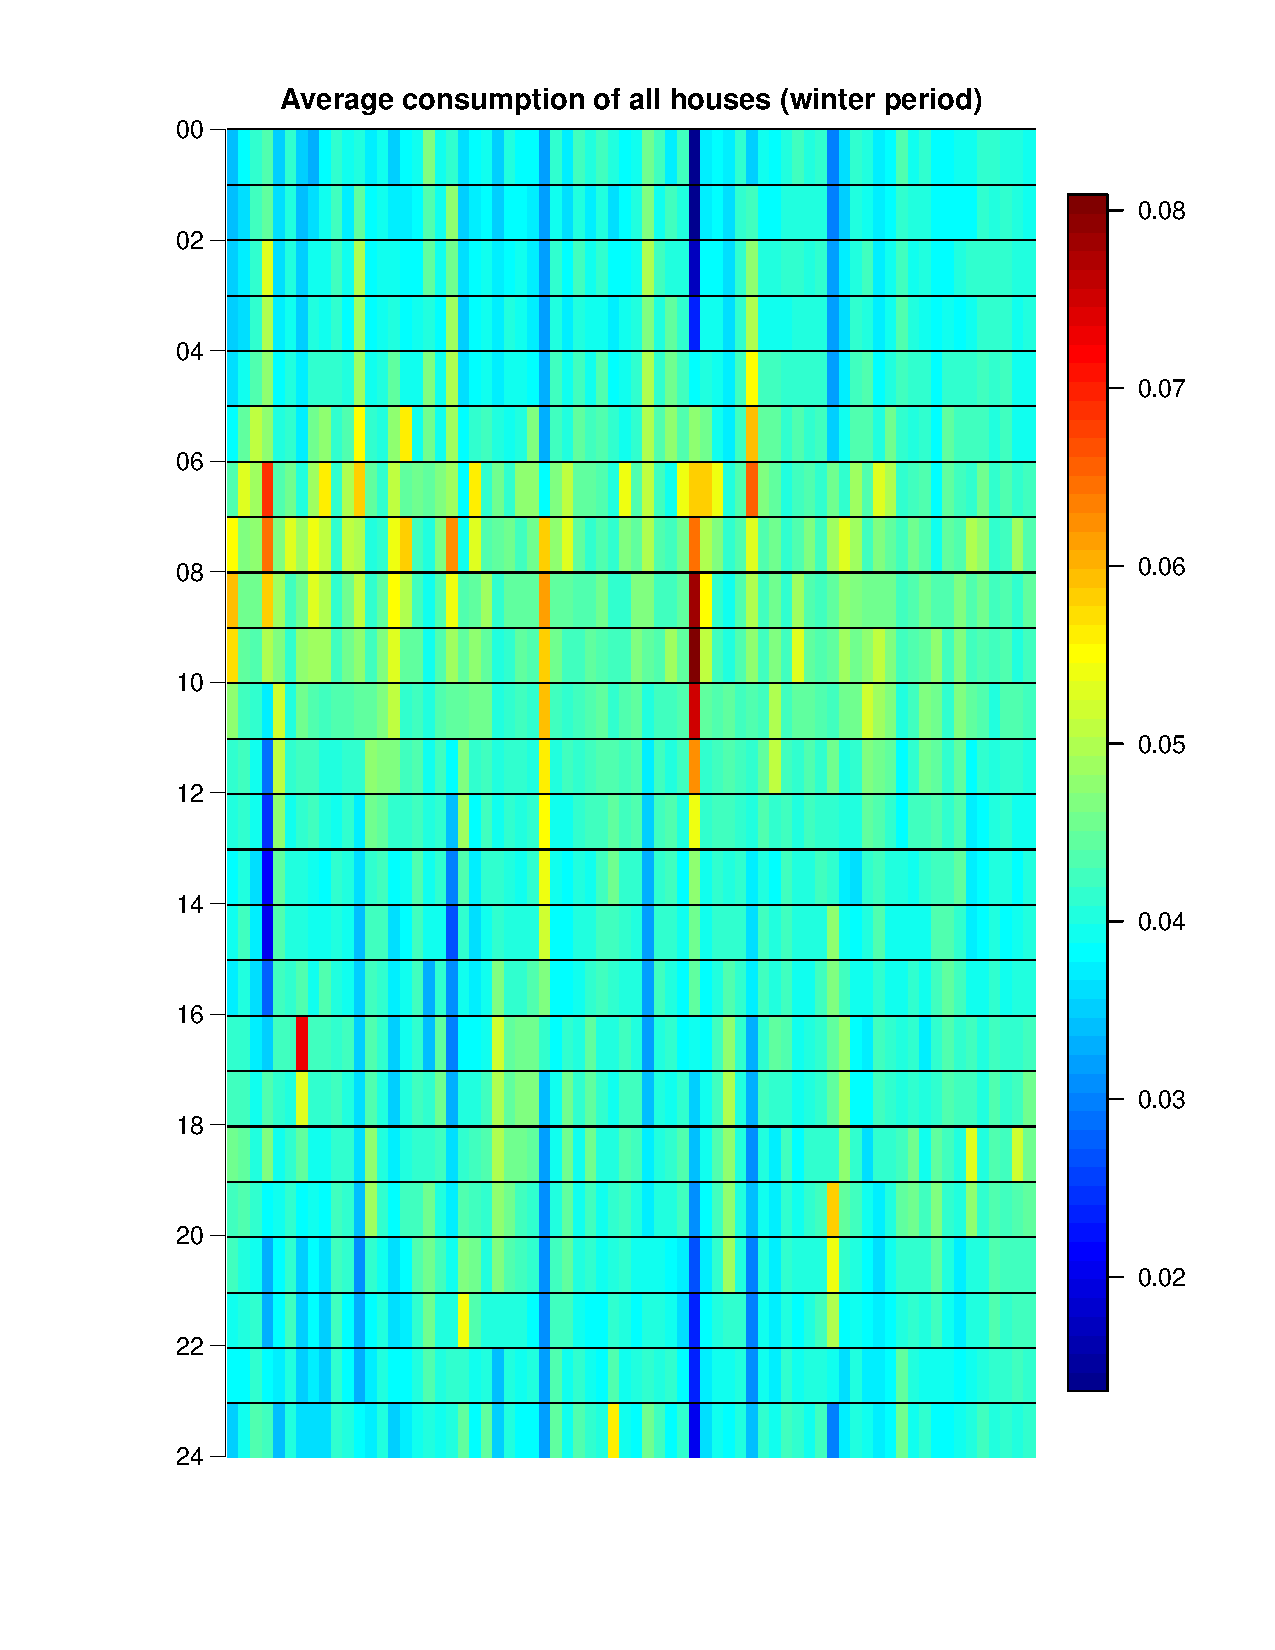
\includegraphics[width=\textwidth]{../../../figures/Heatmap_winter.pdf}
    \caption{This figure shows the same as \cref{fig: daily_cons}, but only in the winter period, characterized by an outside temperature below 12 degrees}
    \label{fig: Hourcons_winter}
\end{figure}

%
\section{Description of the Hourly Consumption}
\noindent \cref{fig: Hourcons_summer} and \cref{fig: Hourcons_winter} show the average consumption of each house during the day for the summer period and the winter period respectively. The different hours can be seen on the y-axis, and the colour coding show the fraction of that house's consumption in that hour interval. Each vertical strip of colours is a single house. Each strip sum up to $1$. Looking at the summer period in \cref{fig: Hourcons_summer}, a generel trend is apparent: the consumption is usually larger around $7$ AM and to some degree around $7$ PM. Almost every house peaks in one of these periods, and some peaks go up to $12\%$ of the daily consumption. On the other hand, there is almost no consumption between $11$ PM and $5$ AM. The same goes for the afternoon between $1$ PM and $4$ PM. \cref{fig:HourDistribution} shows the average distribution of all houses together with lines indicating the quantiles. On the figure it can be seen that the intervals $06-11$ and $18-19$ are in the top quantile. $00-05$ and $15-16$ is where the consumption is lowest.

\noindent These trends make sence. In the summer period, not much energy is used for heating the house. There is usually a significant amount of tap water consumption in the morning, when people take warm baths and make breakfast. Sometimes a dishwasher might be running as well. Then there is not much consumption while people are at work or school. When they get home in the late afternoon the consumption rises again as they prepare for dinner or use hot water in other ways. During the night time the consumption becomes low again.



\noindent The winter period on \cref{fig: Hourcons_winter} is a bit different. There are still significant peaks in the morning, and to some extent in the evening as well, but in general the consumption is more spread out on the entire day. This is mostly because of the heating consumption in the winter period. While people are not at home or while they are sleeping, the heating is still turned on. The highest peaks only go to $8\%$ of the daily consumption here. One house stands out in this plot. A bit to the left of the middle there is a house where the consumption is several times higher between $8$ AM and $12$ noon. This house has almost no consumption during the night. But the house is not a commercial building and its area is only 138 $m^2$. So this house appears to have an efficient night time drop for their thermostat.


\noindent These figures illustrate the general trend of the houses, but it is hard to compare them in a meaningful way. But \cref{fig: Season_dist} shows the average distribution of all houses during the day. Both the winter season and the summer season show the same trends that was discussed above. But this plot also shows how the winter period is more smoothed out than the summer period. Keep in mind that the lines only show the relative distribution, and they do not take into account that the consumption in the winter period is significantly higher. As one can see on the y-axis, the difference between the two curves is very small. A night time period can be defined as the hours $23-05$. This is the period after the consumption drops in the evening, and before it rises in the morning. In this period, the houses on average use $21,9\%$ of their daily consumption in the summer period, and $23,7\%$ in the winter period. A completely uniform consumption would be $25\%$. It is not surpricing that the consumption in the night hours is lower than the average. Neither is it surpricing that the consumption at night in the summer period is relatively smaller than in the winter period. The extra cost of heating the house makes the consumption more spread out on the 24 hours of the day. But it is surpricing that the difference between the summer period and the winter period is only $1.8$ percentage points. With this in mind, the time series modelling will now be introduced. 

\noindent In addition, \cref{fig:HourDistribution} is used to detect the significant intervals during a day in relation to the consumption. It is clearly seen that the time interval with highest consumption is 06-11 am and around 6 pm. \textcolor{red}{Not done}

\begin{figure}
    \centering
    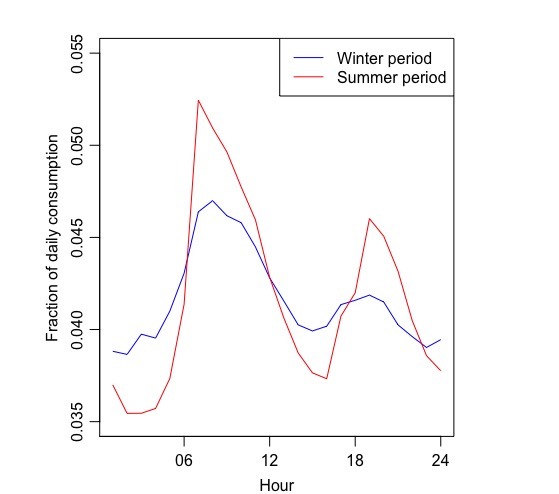
\includegraphics[width=0.7\textwidth]{../../../figures/Season_distribution.jpeg}
    \caption{The average distribution of the heat consumption during the day for the winter period and the summer period respectively. The winter period is more smoothed out, but they are very similar}
    \label{fig: Season_dist}
\end{figure}

\begin{figure}
    \centering
    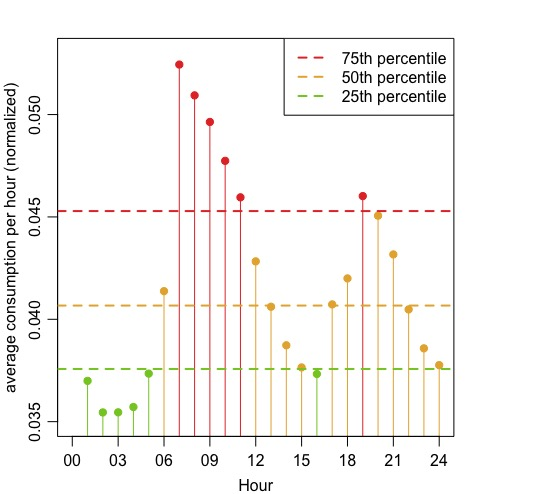
\includegraphics[width=0.8\textwidth]{../../../figures/HourDistribution.jpeg}
    \caption{The average consumption of all houses during the day. Each point indicate the average consumption in the previous hour interval. The hours in the 75th percentile is $06-11$ and $18-19$}
    \label{fig:HourDistribution}
\end{figure}


\section{The ARMA Models and Their Extensions}
The consumption of a house during a certain period with hour intervals is a time series. A time series is a realization of a stochastic process. In this section the ARMA model will be introduced, and an extended ARMA model, the ARIMAX model, will be fitted to the consumption. The theory of the ARMA model is based on chapter 5 from the book "Time Series Analysis" by Henrik Madsen \cite{Time_Series_Analysis}. The ARMA model fits the data to a linear stochastic process, with an autoregression part (AR) and a moving average part (MA). A linear process $\{Y_t\}$ is a process that can be written as
\begin{equation}
    Y_t - \mu = \sum_{i=0}^{\infty} \psi_i \epsilon_{t-i}, \label{linearProcess}
\end{equation}
where $\mu$ is the mean of the process, $\{\epsilon_i\}$ is white noise and $\{\psi_i\}$ is the weights. For now, the mean $\mu$ is assumed to be zero. To define the ARMA model, the backwards shift operator $B$ is first introduced as $B(Y_t) = Y_{t-1}$. An ARMA process has the form
\begin{equation}
    \phi (B)Y_t = \theta (B) \epsilon_t,
\end{equation}
where $\phi$ and $\theta$ are polynomials on the shift operator B with degree $p$ and $q$ respectively. $\theta(B)$ is the autoregressive part and $\phi(B)$ is the moving average part. The process is denoted as an $ARMA(p,q)$ process. ARMA processes are linear. If one applies $\psi(B)$ to $Y_t$ and substitutes $Y_{t-1}$, then $Y_{t-2}$ and so forth, the form in \cref{linearProcess} is obtained.

\noindent An ARMA process is stationary if all the roots of $\phi(z^{-1})$ are within the unit circle. Stationarity is a very desirable property. In a stationary process, the mean and variance does not change over time. But often, processes will not be stationary due to long term trends. For example the mean consumption of a house has a periodic trend during the year. This was clearly illustrated on \cref{fig: daily_cons}. But long term trends can be eliminated by introducing differencing. Instead of modelling the process $\{Y_t\}$, one can model the process $\{Y_t - Y_{t-1}\}$, i.e. the difference between observations. This is formalized with the difference operator $\Delta = (1-B)$. The differenced ARMA model is called the $ARIMA(p,d,q)$ model, or the autoregressive \textit{integrated} moving average model. It has the form
\begin{equation}
    \phi (B) \Delta^d Y_t = \theta (B) \epsilon_t,
    \label{ARIMA}
\end{equation}
where $d\in \mathbb{N}$ is the differencing factor. Apart from the long term trends, the model might also have short term periodic trends. In this case a 24 hour periodic trend would be expected. The ARIMA model can be expanded to a seasonal ARIMA with season $s$, such that
\begin{equation}
    \phi (B) \Phi (B^s) \Delta^d \Delta_s^D Y_t = \theta (B) \Theta (B^s) \epsilon_t.
    \label{eq:ARIMA}
\end{equation}
This is a seasonal $ARIMA(p,d,q)\times (P,D,Q)_s$. $\phi$, $B$, $\Delta$ and $\theta$ are defined as in \cref{ARIMA}. But here $\Phi$ and $\Theta$ are also included. They are polynomials in $B^s$ of degree $P$ and $Q$ respectively. $D$ is the differencing of the seasonal component of the model. 

\noindent In this particular project we have access to the consumption, but also to the weather data. The exploratory analysis showed that there was a significant correlation between consumption and temperature. The temperature is also a time series, and it can be used as input to the ARIMA model to make a better fit. This is called using an exogenous variable. When an exogenous variable is used, the model is called an ARIMAX model. The following part is based on chapter $8$ in \cite{Time_Series_Analysis} and the $R$ documentation. The model looks like this


\begin{equation}
    \phi (B) \Phi (B^s) \Delta^d \Delta_s^D Y_t = \theta (B) \Theta (B^s) \epsilon_t + \omega(B) X_t,
    \label{eq:ARIMAX}
\end{equation}
where $X_t$ is the exogenous variable and $\omega(B)$ is a polynomial in $B$. The exogenous part can also be differenced or have seasonal components, but in this project those extensions will not be explored. In fact only $\omega(B)=\omega_0$ will be used in the modelling process. The software used for the arima processes is of course $R$, but in particular the $arima$ function. This function does not estimate the exogenous parameters according to \cref{eq:ARIMAX}. It actually starts out by making a regression of the series $\{Y_t\}$ on the exogenous variable $\{X_t\}$. Then this fit is substituted for $Y_t$ in \cref{eq:ARIMA}. This approach is less precise, since it executes the parameter estimation in two steps, first for the exogenuous variable, then for the rest of the variables. An alternative method is to use the \texttt{MARIMA} package in \texttt{R}. This package computes the estimates in \cref{eq:ARIMAX} by using different approximation methods than the \texttt{arima} function. Neither methods should be considered "correct", but they produce different results.

\section{Applying the models}
In this section, different ARIMAX models will be applied to the data. First the \texttt{arima} function in \texttt{R} will be used to test different models. The models will include a season of 24 hours. Then the chosen model will be compared with the /\texttt{MARIMA} function. In the next section the models will be used to make predictions on the data.

\textcolor{red}{Vi bruger både sommer og vinter. Temperaturen er lavet om til antal grader under 12.}

\subsection{Modelling with the $arima$ Function}
To generate a model, one must decide a model order. It is important that the model is not too complex. With the amount of data available for each house, too many parameters in the model causes the running time to increase drastically. More importantly, sometimes the optimization method used in the $arima$ function does not converge. This happens more often when there are more parameters, and the model should be applicaple to as many different houses as possible. As mentioned in the section above, stationarity is an important property. If the order of the autoregressive part (both non-seasonal and seasonal) is too high, the model will not be stationary unless differencing is used. Differencing on the other hand makes the model more obscure and harder to interpret. If the model is only differenced once, it means that it models the difference between one hour and the one before that. If the seasonal part is differenced, it models the difference between an hour and the same hour the day before.

\noindent These considerations have led to the conclusion that a $(1,0,1)\times (1,0,1)$ model is a good starting point. Written in the form of \cref{eq:ARIMA} it is
\begin{equation}
    (1-\phi_1 B)(1-\Phi_1 B^{24})Y_t = (1+\theta_1 B)(1+\Theta_1 B^{24}) \epsilon_t. \label{eq:model1}
\end{equation}
The negative sign of the $\phi$ values is due to the convention of the $arima$ function, where $Y_t$ is isolated to one side of the equation. The model can also be formulated as
\begin{align}
    Y_t = &\phi_1 Y_{t-1} + \Phi_1 Y_{t-24} + \phi_1 \cdot \Phi_1  Y_{t-25}\\  &+ \theta_1 \epsilon_{t-1} + \Theta_1 \epsilon_{t-24} + \theta_1 \cdot \Theta_1 \cdot \epsilon_{t-25} + \epsilon_t. \nonumber
\end{align}

\noindent For most houses this model is not stationary and the optimization does not converge. \cref{fig:Model1_stationarity} shows the roots of the model when applied to house 55. On the left the AR roots are illustrated, on the right the MA roots are illustrated. When considering stationarity, only the AR roots are of interest. Here it can be seen how every inverse AR root is on the edge of the unit circle. This model introduces $25$ roots in $\phi$, $1$ from the non-seasonal part, and $24$ from the seasonal part. As many of the inverses of these roots as possible should be inside the unit circle. For this reason, it makes the most sence to difference the seasonal part of the model. The one root from the non-seasonal part might still be on the edge of the unit circle, but the rest will most likely not be.

\begin{figure}
    \centering
    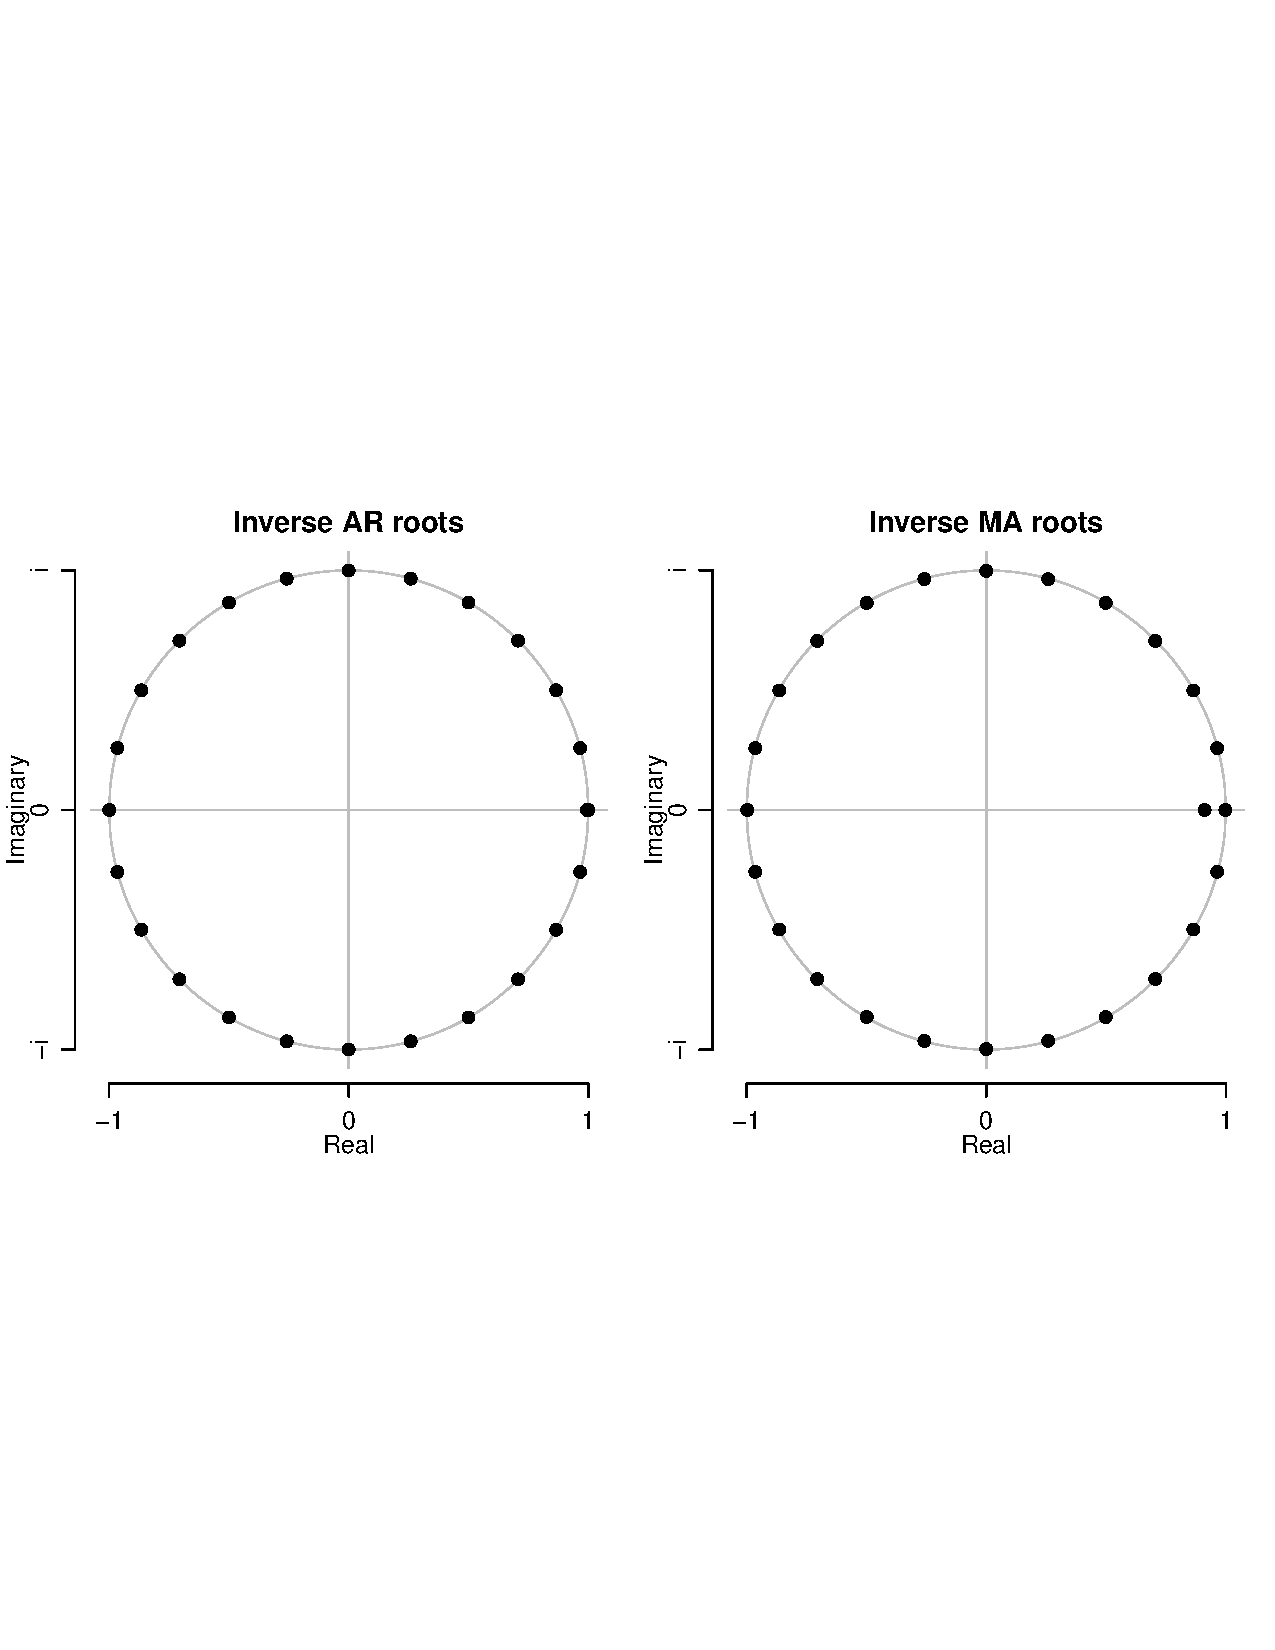
\includegraphics[width=0.8\textwidth]{../../../figures/arimax/Stationarity_model1.pdf}
    \caption{The roots of the first model when applied to house 55. All the inverse AR roots are on the edge of the unit circle}
    \label{fig:Model1_stationarity}
\end{figure}

\noindent Thus, the next model is a $(1,0,1)\times(1,1,1)$ model, written as
\begin{equation}
    (1-\phi_1 B)(1-\Phi_1 B^{24})(1-B^{24})Y_t = (1+\theta_1 B)(1+\Theta_1 B^{24}) \epsilon_t.
\end{equation}
This is the same model as in \cref{eq:model1}, except for the differencing. When rewritten, the model becomes:
\begin{align}
    Y_t-Y_{t-24} = &\phi_1 (Y_{t-1}-Y_{t-25}) + \Phi_1 (Y_{t-24}-Y_{t-48}) + \phi_1 \cdot \Phi_1  (Y_{t-25}-Y_{t-49}) \label{model101111}\\  &+ \theta_1 \epsilon_{t-1} + \Theta_1 \epsilon_{t-24} + \theta_1 \cdot \Theta_1 \cdot \epsilon_{t-25} + \epsilon_t. \nonumber
\end{align}
This shows clearly how the model now operates on the difference between a value and the same value a day earlier. Firstly, the stationarity of this model should be evaluated. The inverse roots of house 55 and 18 are shown in \cref{fig:Model2_stationarity55} and \cref{fig:Model2_stationarity18} respectively. For house 55 the 24 seasonal AR roots are within the unit circle. The last root is not. While this is not optimal, it is definitely better than the last model without differencing. For house 18 all the roots are sufficiently within the unit circle. This is true for most of the houses the model was applied to. So in terms of stationarity the model performs well over all. It would be better to introduce non-seasonal differencing as well, but to keep the model simple no further differencing is applied.


\begin{figure}
    \centering
    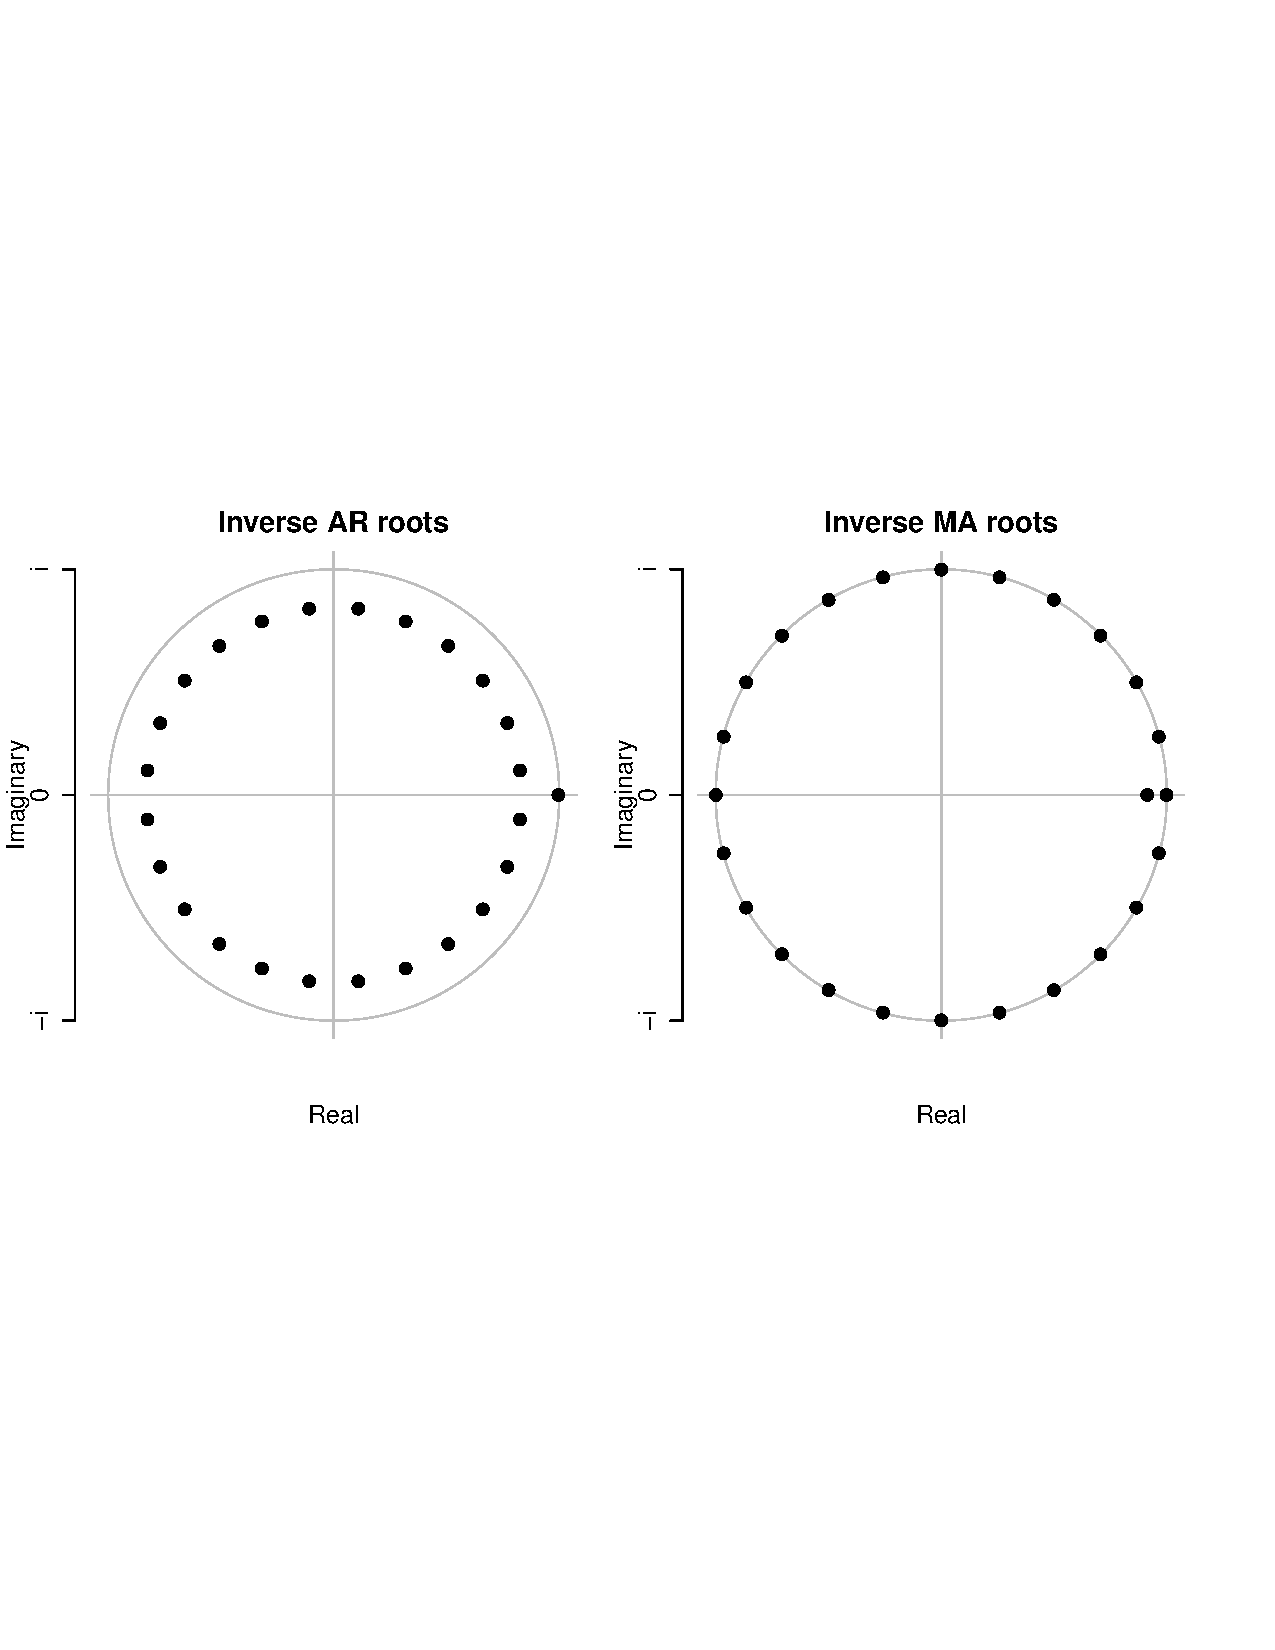
\includegraphics[width=0.8\textwidth]{../../../figures/arimax/Roots_55.pdf}
    \caption{The roots of the second model when applied to house 55.}
    \label{fig:Model2_stationarity55}
\end{figure}    


\begin{figure}
    \centering
    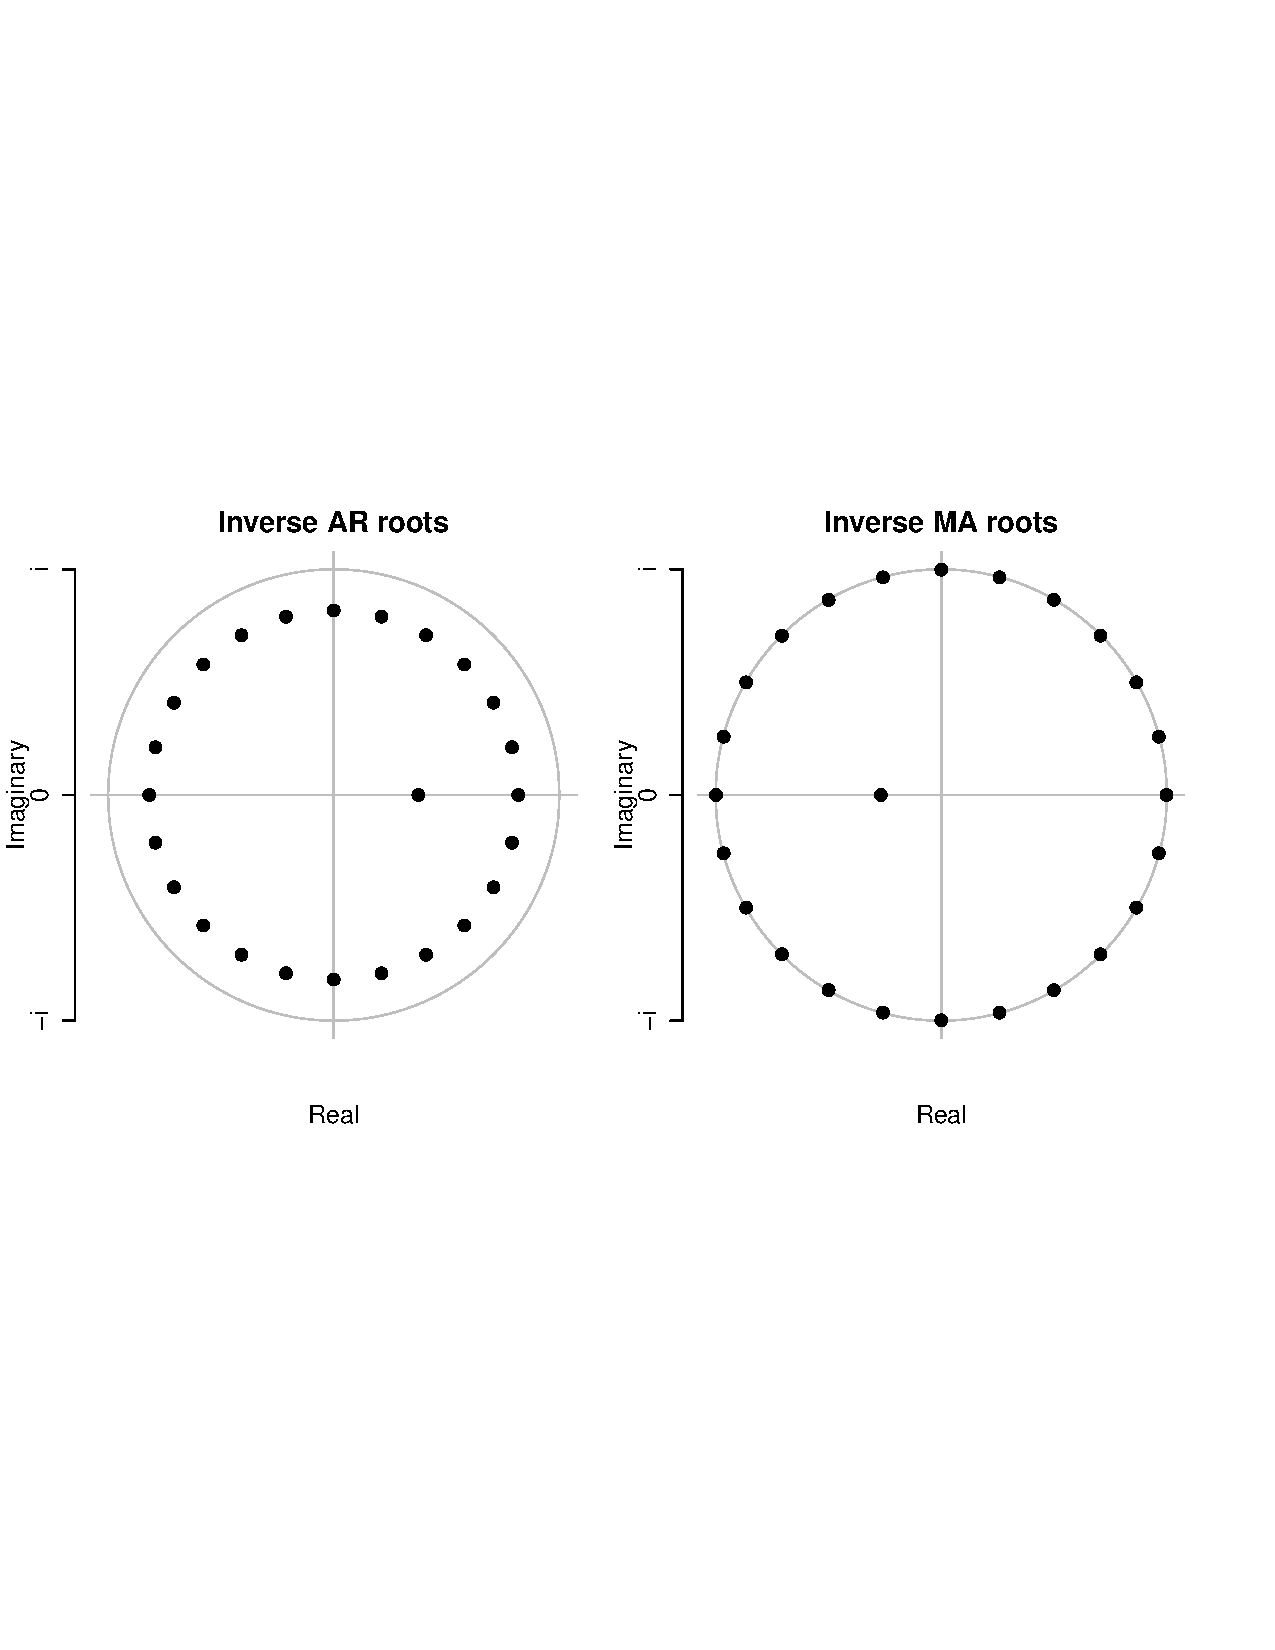
\includegraphics[width=0.8\textwidth]{../../../figures/arimax/Roots_18.pdf}
    \caption{The roots of the second model when applied to house 18.}
    \label{fig:Model2_stationarity18}
\end{figure}    

\noindent After considering the stationarity of the model, the significance of the parameters is examined. The model is applied to $70$ houses, making it hard to evaluate based on a few houses. \cref{tab:ParamSig_Model1} gives an overview of how many models have significant parameters. It shows how many of the houses have parameters below two and three standard deviations respectively. It can be seen that the seasonal AR1 is the parameter that is most often not significant. For $36$ of the houses the parameter value is below two standard deviations, which is about half of the houses. For $50$ of the houses, the parameter is below three standard deviations, so most of them are not significant, or barely significant. Looking specifically at house 55, the parameter values and standard deviations are listed in \cref{tab:ParamSig_House55}. Here the seasonal AR is only just a little bit bigger than the standard deviation, making it insignificant. If the estimates were inserted into \cref{model101111}, one would get the equation
\begin{align}
    Y_t-Y_{t-24} = &0.9949 (Y_{t-1}-Y_{t-25}) - 0.0122 (Y_{t-24}-Y_{t-48}) - 0.0121  (Y_{t-25}-Y_{t-49}) \\  &- 0.9124 \epsilon_{t-1} -0.9572 \epsilon_{t-24} + 0.8733 \epsilon_{t-25} + \epsilon_t. \nonumber
\end{align}
This is after regression with the temperature has been substituted for the $Y_t$. The autocorrelation function (acf) and the partial autocorrelation function (pacf) for this model is visualized in \cref{fig:Model2_acf_55}. There are clearly some significant spikes on the first couple of lags, both in the acf and in the pacf. There are also a few significant lags scattered out on the rest of the function. It should also be noted that the lags around the seasons, indicated by the red lines, do not stand out. The model clearly has problems in the first couple of lags, where there is autocorrelation between the residuals. On the other hand the seasons seem to be accounted for. The rest of the significant lags are relatively random and not very significant. They could be regarded as white noise. The pacf show signs of some oscilleration, but it might just be some distortion in the model. To get a view of the long term effects, \cref{fig:Model2_acf_55_long} in the appendix show the acf and the pacf for an entire week. Here it is still clear that the model is far from perfect, but the biggest issue is the first couple of lags. After that, none of the lags reach more than about $0.05$, which is acceptable. One lag of particular interest is the one at the last red line. This is lag $168$ (the seventh season), which is the autocorrelation between weeks. It shows the autocorrelation between the current residual and the same residual one week earlier. A high autocorrelation in lag $168$ could be a threat to the performance of the model. Fortunately, no lags around this season seem to stand out for house $55$. So for this model the effect between weeks, which is not taken into account, does not seem to have much influence. If one were to try to adress the high correlation in the first lags, the non-seasonal part of the model could be expanded with a higher degree of either AR or MA.


\begin{table}[]
    \centering
    \begin{tabular}{l|ccccc}
    \hline
    \textbf{Parameters} & \textbf{AR1} & \textbf{MA1} & \textbf{SAR1} & \textbf{SMA1} & \textbf{Temperature} \\ \hline \hline
    Below 2 sd & 0   & 3   & 36   & 0    & 6           \\ 
    Below 3 sd & 0   & 3   & 50   & 0    & 14          \\ \hline
    \end{tabular}
    \caption{The number of houses where each parameter is below two standard deviations and three standard deviations respectively. The $(1,0,1)\times (1,1,1)$ model was applied to $70$ houses in total. The average log likelihood of the model is $-6999$}
    \label{tab:ParamSig_Model1}
\end{table}

\begin{table}[]
    \centering
    \begin{tabular}{l|ccccc}
    \hline
    \textbf{House 55} & \textbf{AR1} & \textbf{MA1} & \textbf{SAR1} & \textbf{SMA1} & \textbf{Temperature} \\ \hline \hline
    Estimate           & 0.9949 & -0.9124 & -0.0122 & -0.9572 & 0.0288      \\ 
    Standard deviation & 0.0013 & 0.0048  & 0.0111  & 0.0043  & 0.0045      \\ \hline
    \end{tabular}
    \caption{The estimates of the parameters for the $(1,0,1)\times (1,1,1)$ model together with their standard deviations for house 55. The log likelihood of the model is $-5791$}
    \label{tab:ParamSig_House55}
 \end{table}

 \begin{figure}
    \centering
    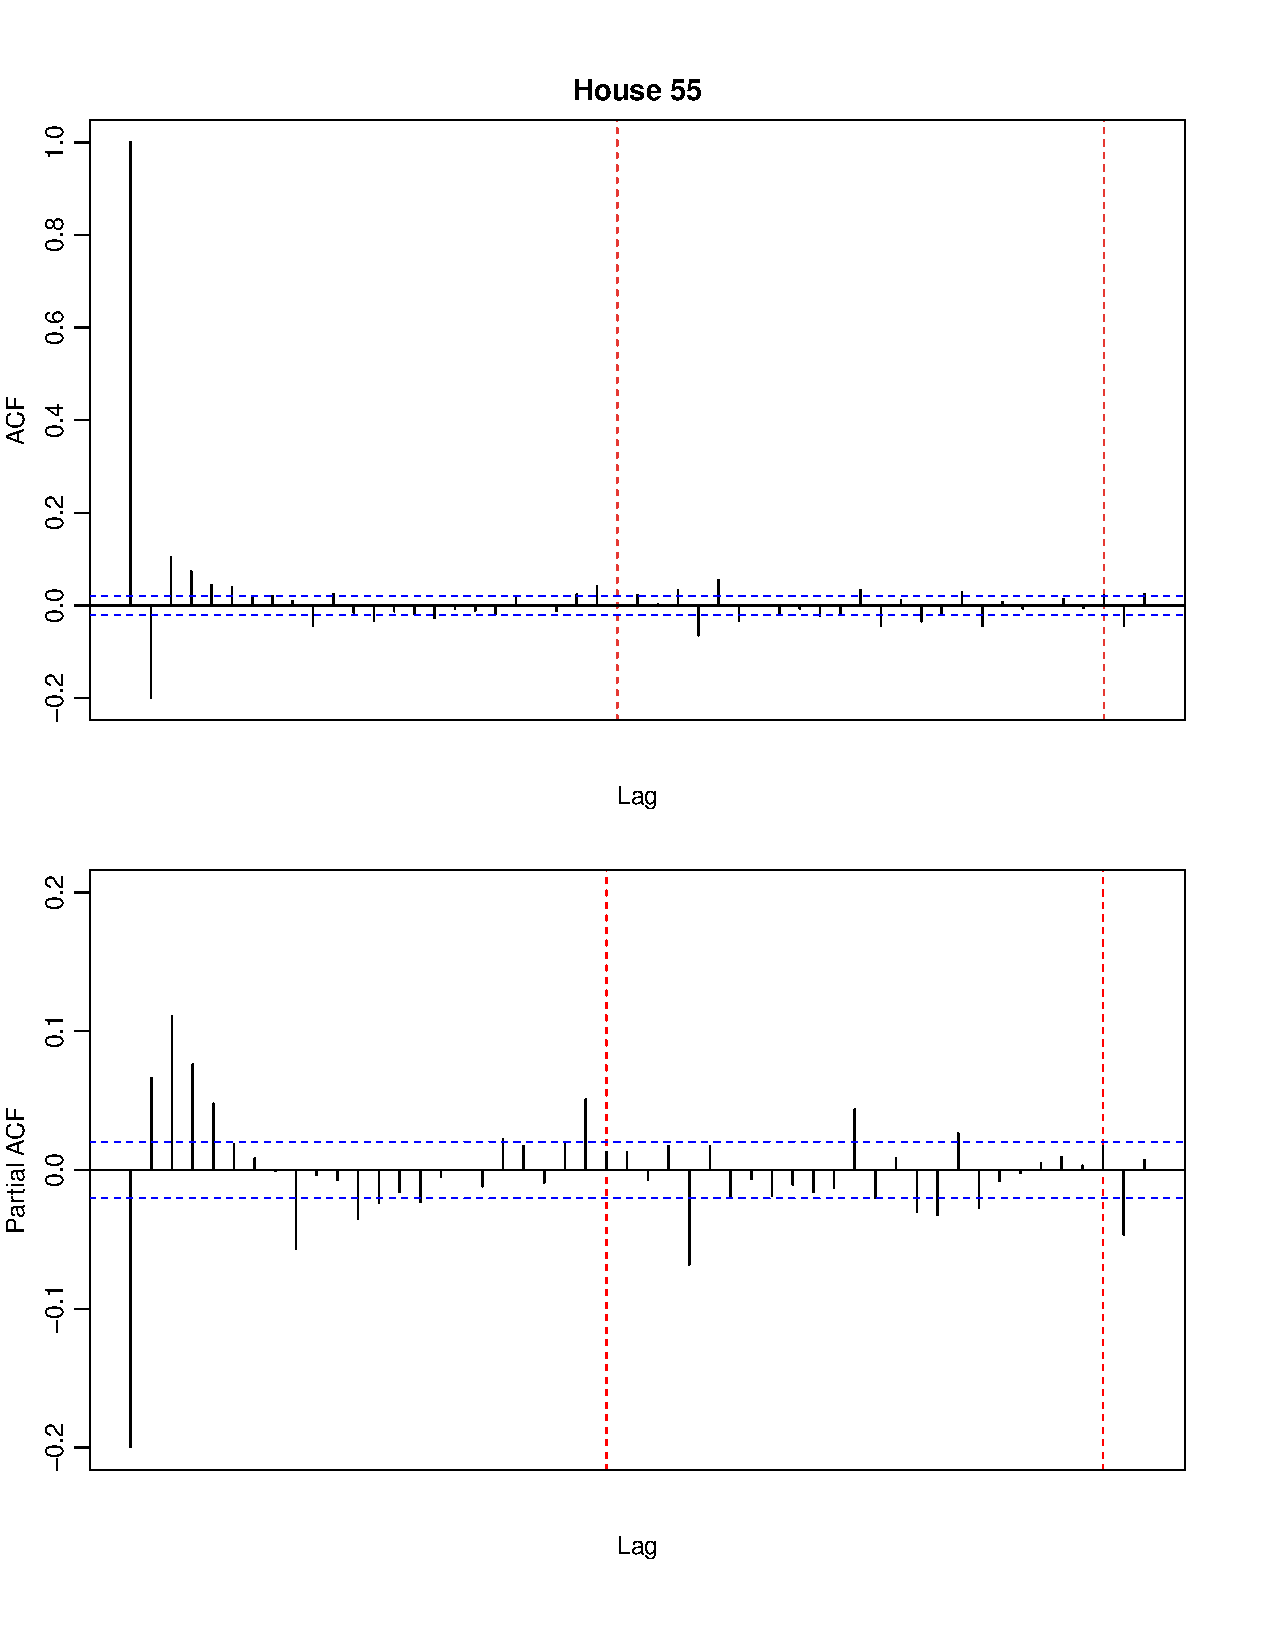
\includegraphics[width=0.8\textwidth]{../../../figures/arimax/ACF_55_short.pdf}
    \caption{The acf and pacf of the second model when applied to house 55. The 24 hour seasons are highlighted with red dashed lines. The blue lines indicate the 95\% confidence interval}
    \label{fig:Model2_acf_55}
\end{figure}    


\noindent Now the model will be evaluated for house 18. The estimates for the model are listed in \cref{tab:ParamSig_House18}. Here the seasonal AR1 is even more insignificant than it was for house 55, being less than the standard deviation. The log likelihood of the model for this house $(-12780)$ is also much lower than for house 55 $(-5791)$, or than the average of the model $(-6999)$. After insertion into \cref{model101111} the model for house 18 is
\begin{align}
    Y_t-Y_{t-24} = &0.3751 (Y_{t-1}-Y_{t-25}) + 0.008 (Y_{t-24}-Y_{t-48}) + 0.003 (Y_{t-25}-Y_{t-49}) \\  &+ 0.2672 \epsilon_{t-1} - 0.9559 \epsilon_{t-24} - 0.2554 \epsilon_{t-25} + \epsilon_t. \nonumber
\end{align}
This is again after the regression fit with the temperature has been substituted for $Y_t$. Looking at the acf and pacf of this house on \cref{fig:Model2_acf_18}, this house does not have the same high autocorrelation in the first lags. Actually both the acf and the pacf look slightly better for house 18 than they did for house 55, even though house 18 overall has shown unpredictable behavior. There are still significant lags in both the acf and the pacf, but as for house 55, they are not very large and can to some extent be regarded white noise. As for the 24 hour seasons, there are no significant outliers. There is no pattern indicating that the residuals for the 24 hour seasons are not sufficiently accounted for in the model. When looking at \cref{fig:Model2_acf_18_long} in the appendix where an entire week is included, there is a single peak at season four that stands out. But since the other seasons do not show the same behavior, it might as well be a coincidence. Just like for house 55 there is no significant peak at the seventh season. Overall, even though there are many significant peaks in both the acf and the pacf, there is no obvious pattern connected to the seasons or the first lags. And none of the peaks reach a value higher than $0.1$.

 \begin{table}[]
    \centering
    \begin{tabular}{l|ccccc}
    \hline
    \textbf{House 18} & \textbf{AR1} & \textbf{MA1} & \textbf{SAR1} & \textbf{SMA1} & \textbf{Temperature} \\ \hline \hline
    Estimate           & 0.3751 & 0.2672 & 0.008 & -0.9559 & 0.0825      \\ 
    Standard deviation & 0.0171 & 0.0175 & 0.011 & 0.0040  & 0.0078      \\ \hline
    \end{tabular}
    \caption{The estimates of the parameters for the $(1,0,1)\times (1,1,1)$ model together with their standard deviations for house 18. The log likelihood of the model is $-12780$}
    \label{tab:ParamSig_House18}
    \end{table}


\begin{figure}
    \centering
    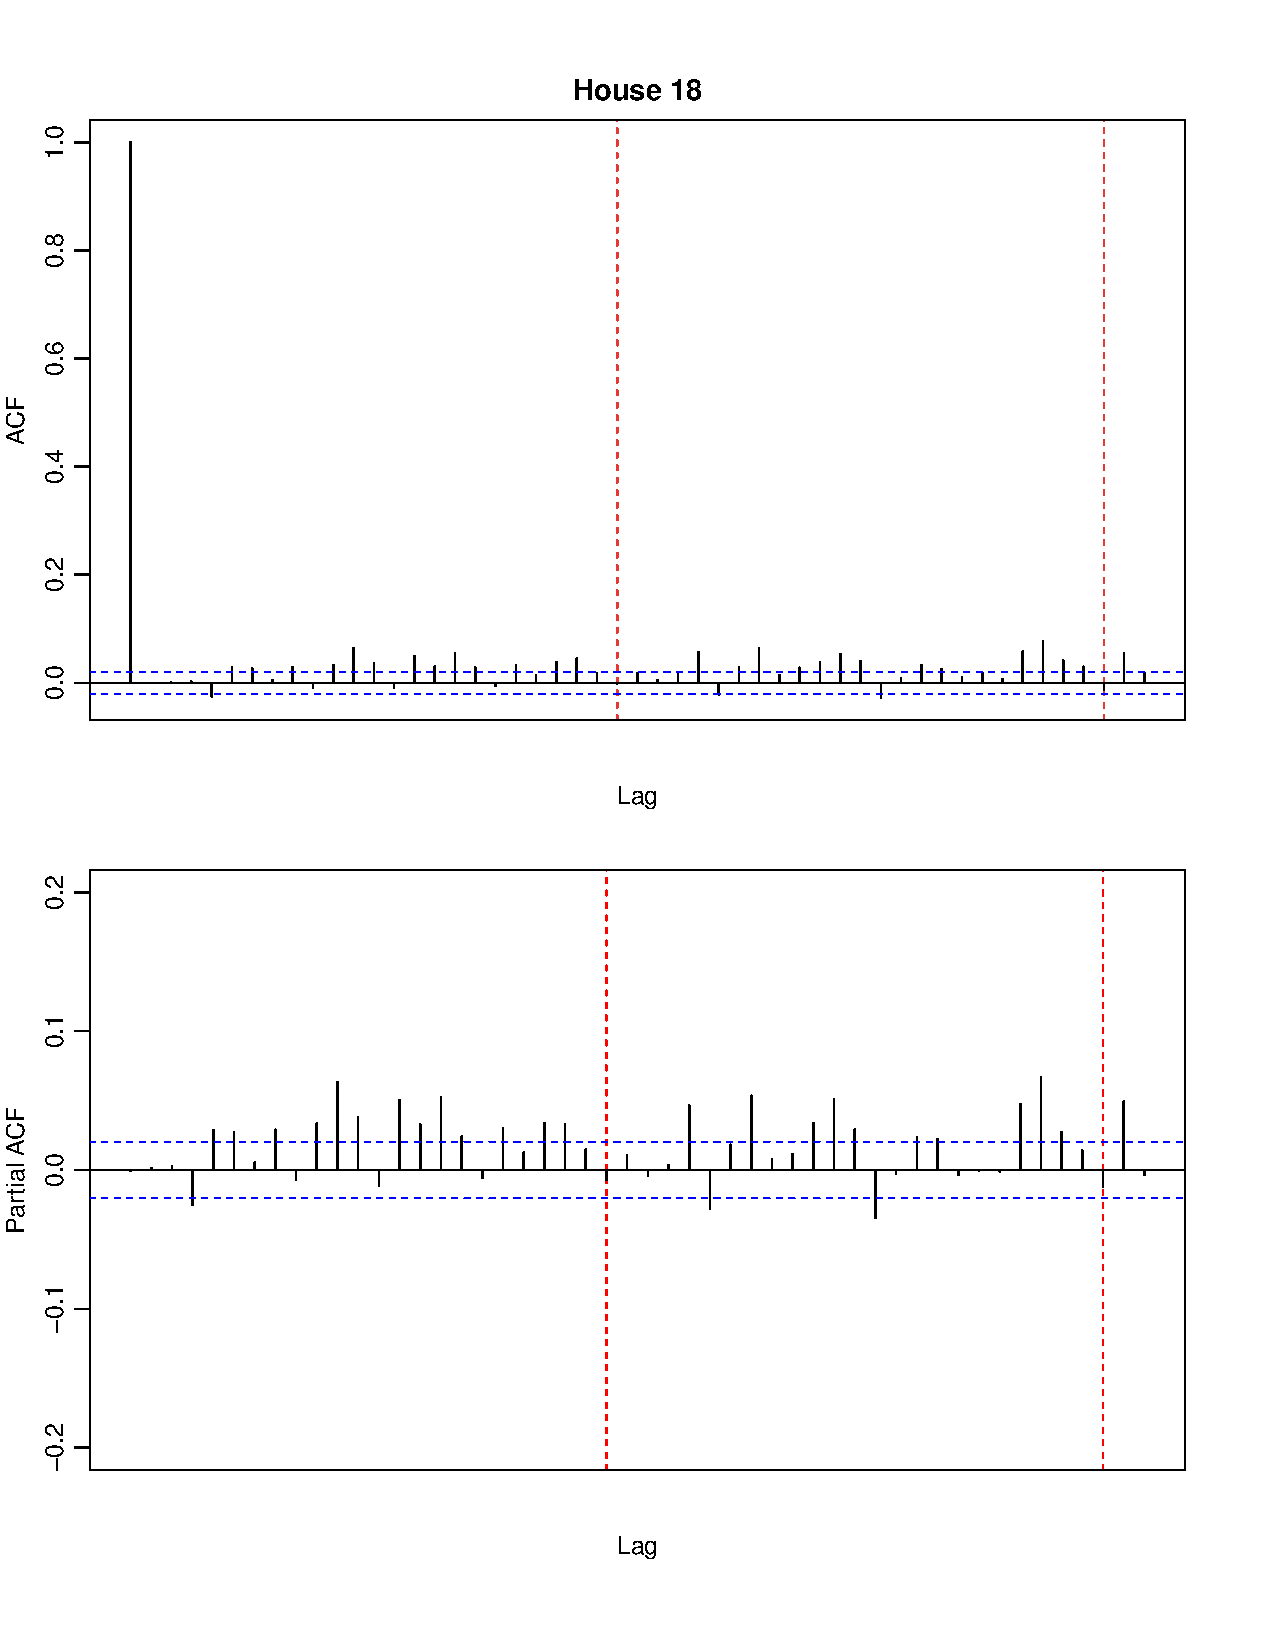
\includegraphics[width=0.8\textwidth]{../../../figures/arimax/ACF_18_short.pdf}
    \caption{The acf and pacf of the second model when applied to house 18. The 24 hour seasons are highlighted with red dashed lines. The blue lines indicate the 95\% confidence interval}
    \label{fig:Model2_acf_18}
\end{figure}    







\subsection{Modelling with the MARIMA Function}




\section{Making Predictions}

\section{Visualization of the results} 

